\subsection{Differential Equations and Initial Value Problems}

Differential equations are used to:
\begin{enumerate}
  \item Model physical situations.
  \item Solve the resulting equations.
  \item Interpret the solutions.
\end{enumerate}

\begin{definition}{Ordinary Differential Equation}{ordinary-differential-equation}
  \begin{center}
    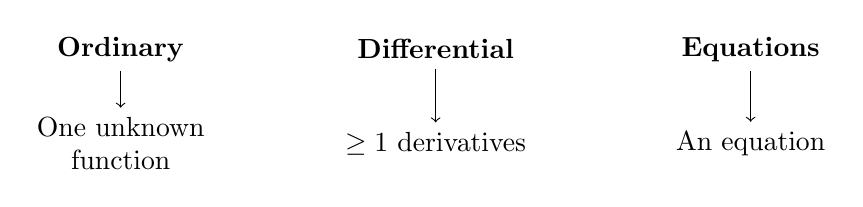
\begin{tikzpicture}
      \node (ordinary) at (0,0) {\textbf{Ordinary}};
      \node (differential) at (4,0) {\textbf{Differential}};
      \node (equations) at (8,0) {\textbf{Equations}};
      \node[align=center] (unknown) at (0,-1.2) {One unknown\\function};
      \node[align=center] (derivatives) at (4,-1.2) {$\geq 1$ derivatives};
      \node (equation) at (8,-1.2) {An equation};
      \draw[->] (ordinary) -- (unknown);
      \draw[->] (differential) -- (derivatives);
      \draw[->] (equations) -- (equation);
    \end{tikzpicture}
  \end{center}
  Here, \emph{ordinary} specifies that the unknown function depends on one independent variable.
\end{definition}

\begin{example}[Solving by Integration]
  Solve
  \[
    \frac{dy}{dx}=x^2.
  \]
  Integrating gives
  \[
    y(x)=\frac{x^3}{3}+C, \qquad C\in\R.
  \]
\end{example}

\begin{definition}{Order of an ODE}{ode-order}
  The \textbf{order} of an ODE is the order of the highest derivative appearing in the equation.
\end{definition}

\begin{definition}{Initial Condition}{initial-condition}
  An \textbf{initial condition} specifies a value that a solution (or one of its derivatives) must satisfy at a given point. For example, $y(a)=b$ requires the solution to pass through $(a,b)$.
\end{definition}

\begin{definition}{Initial Value Problem}{initial-value-problem}
  An \textbf{initial value problem (IVP)} consists of an ODE together with initial conditions.
\end{definition}

\begin{example}[Determining the Constant]
  Solve the IVP
  \[
    \begin{cases}
      \dfrac{dy}{dx}=x^2, \\
      y(1)=3.
    \end{cases}
  \]
  The general solution is $y(x)=x^3/3+C$. The initial condition gives
  \[
    3=\frac{1}{3}+C \quad\Longrightarrow\quad C=\frac{8}{3}.
  \]
  Thus
  \[
    y(x)=\frac{x^3}{3}+\frac{8}{3}.
  \]
\end{example}

\subsubsection{Direct Integration}

For an equation of the form
\[
  \frac{dy}{dx}=f(x),
\]
the general solution is an antiderivative of $f$:
\[
  y(x)=F(x)+C, \qquad F'(x)=f(x).
\]
If $f$ is continuous, the IVP
\[
  \begin{cases}
    \dfrac{dy}{dx}=f(x), \\
    y(a)=b
  \end{cases}
\]
has solution
\[
  y(x)=b+\int_a^x f(t)\dd{t}.
\]

\begin{example}[Identifying the Order]
  The equation
  \[
    \frac{d^2y}{dx^2}+3\frac{dy}{dx}+7y=e^x
  \]
  is a second-order ODE, since its highest derivative is $d^2y/dx^2$.
\end{example}

\subsubsection{An Equation Involving the Unknown Function}

\begin{example}[Exponential Growth]
  Solve the IVP
  \[
    \begin{cases}
      \dfrac{dy}{dx}=y, \\
      y(1)=7.
    \end{cases}
  \]
  For $y\ne0$, viewing $x$ as a function of $y$ gives (can also integrate by partial fraction and substitution)
  \[
    \frac{dx}{dy}=\frac{1}{y}.
  \]
  Integrating,
  \[
    x=\ln\abs{y}+C.
  \]
  The initial condition gives $C=1-\ln 7$, so
  \begin{align*}
    x       & = \ln\abs{y}+1-\ln 7,     \\
    \abs{y} & = e^{x+\ln 7-1}=7e^{x-1}.
  \end{align*}
  Since $y(1)=7>0$, the solution is
  \[
    y(x)=7e^{x-1}.
  \]
\end{example}
